\documentclass[12pt,a4paper]{article}
\usepackage[left=4cm,right=3cm,top=3cm,bottom=3cm]{geometry}
\usepackage{mathptmx} % Times New Roman
\usepackage[T1]{fontenc}
\usepackage{textcomp}
\usepackage{amsmath}
\usepackage{amssymb}
\usepackage{graphicx}
\usepackage{float}
\usepackage{hyperref}
\usepackage[none]{hyphenat}
\usepackage{tikz}
\usepackage{enumitem}
\usepackage{titlesec}
\usepackage{multirow}
\usepackage{setspace}
\usepackage{setspace}
\usepackage{ragged2e}

\usepackage{titlesec}

% Pengaturan hyphenation untuk Bahasa Indonesia
\sloppy % Membuat LaTeX lebih fleksibel dengan spacing
\tolerance=9999
\emergencystretch=3em
\hbadness=9999
\hyphenpenalty=10000
\exhyphenpenalty=50
\doublehyphendemerits=10000
\finalhyphendemerits=5000
\pretolerance=100

% Pengaturan paragraf: tanpa indentasi dan jarak minimal antar paragraf
\setlength{\parindent}{0pt} % Menghilangkan indentasi awal paragraf
\setlength{\parskip}{0pt} % Tidak ada jarak antar paragraf

% Pengaturan jarak untuk subsection
\titleformat{\subsection}{\normalsize\bfseries}{\thesubsection}{1em}{}
\titlespacing*{\subsection}{0pt}{0pt}{0pt} % Tidak ada jarak sebelum atau setelah judul

% Pengaturan jarak untuk subparagraph
\titleformat{\subparagraph}[runin]{\normalsize\bfseries}{\thesubparagraph}{1em}{}
\titlespacing*{\subparagraph}{0pt}{0pt}{1em} % Memberikan sedikit spasi setelah judul

% Pengaturan spasi
\onehalfspacing

% Pengaturan penomoran
\renewcommand{\thesection}{\Roman{section}}
\renewcommand{\thesubsection}{\thesection.\arabic{subsection}}
\renewcommand{\thesubsubsection}{\thesubsection.\arabic{subsubsection}}
\renewcommand{\thesubparagraph}{\thesubsubsection.\arabic{subparagraph}}

\begin{document}

\sloppy

\vspace{2cm}
\begin{center}
{\fontsize{14}{16.8}\selectfont\textbf{BAB III. Metodologi Penelitian}}\\[1em]
\end{center}
\label{sec:metodologi}
\addcontentsline{toc}{section}{BAB III METODOLOGI PENELITIAN}
\setcounter{section}{3}
\setcounter{subsection}{0}
\vspace{2em}

Bab ini menguraikan pendekatan penelitian yang mengintegrasikan \textit{Design Science Research Methodology} (DSRM) sebagai kerangka sistematis untuk identifikasi masalah, penetapan tujuan, desain, evaluasi, dan komunikasi hasil penelitian. Metodologi ini dipilih karena kesesuaiannya dengan tujuan penelitian, yaitu merancang, mengembangkan, dan mengevaluasi sebuah artefak berupa framework restorasi dokumen berbasis GAN dengan Dual Modal Diskriminator dan loss function berorientasi HTR. Implementasi teknis framework dilakukan melalui siklus iteratif \textit{deep learning} yang berbasis bukti empiris dan dokumentasi sistematis.
\vspace{1em}
\subsection{Kerangka Design Science Research Methodology (DSRM)}
\label{subsec:dsrm-framework}
\vspace{0.8em}

Design Science Research Methodology (DSRM), yang diperkenalkan oleh Peffers et al. (2007), merupakan framework penelitian yang dirancang khusus untuk pengembangan dan evaluasi artefak teknologi informasi. DSRM terdiri dari enam tahapan yang saling terkait dan bersifat iteratif, di mana hasil dari tahap evaluasi memberikan umpan balik untuk penyempurnaan pada tahap desain dan pengembangan.

\begin{figure}[H]
\centering
% Diagram DSRM Framework - TikZ Flowchart
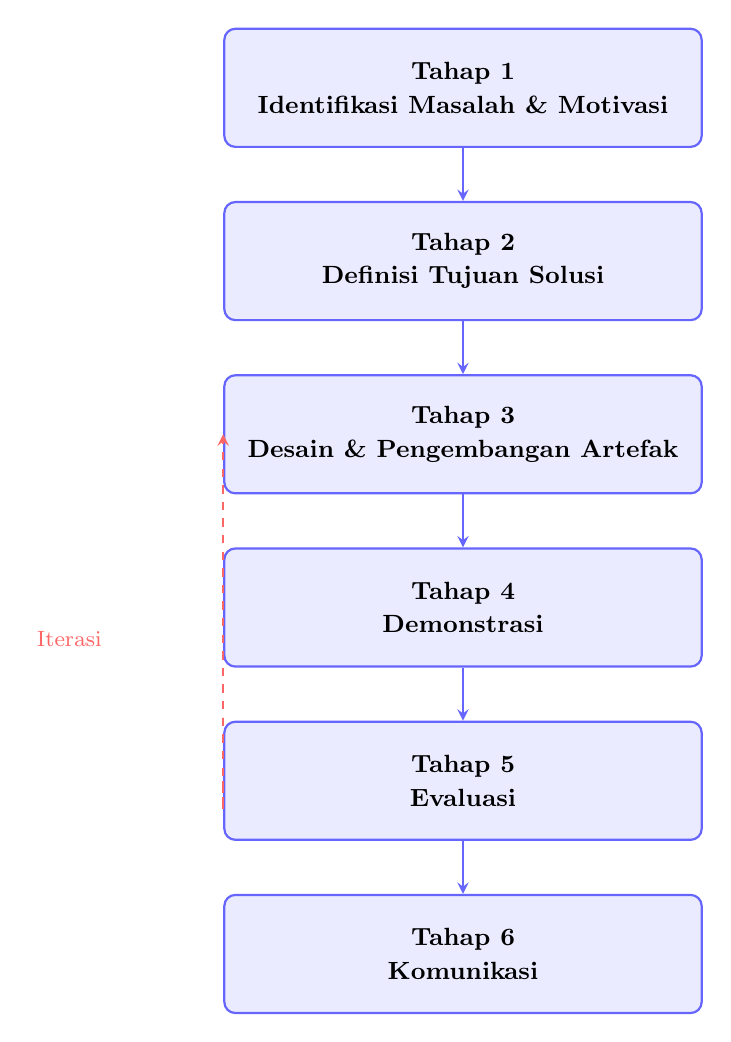
\begin{tikzpicture}[
    node distance=1.2cm,
    box/.style={
        rectangle,
        draw=blue!60,
        thick,
        minimum width=6cm,
        minimum height=1.5cm,
        text centered,
        font=\small\bfseries,
        fill=blue!8,
        rounded corners=4pt,
        inner sep=8pt
    },
    arrow/.style={
        ->,
        thick,
        >=stealth,
        color=blue!60
    }
]

% Phase 1
\node[box] (phase1) at (0,0) {
    \begin{minipage}{5.5cm}
    \centering
    \textbf{Tahap 1}\\
    \vspace{0.1em}
    Identifikasi Masalah \& Motivasi
    \end{minipage}
};

% Phase 2
\node[box] (phase2) at (0,-2.2) {
    \begin{minipage}{5.5cm}
    \centering
    \textbf{Tahap 2}\\
    \vspace{0.1em}
    Definisi Tujuan Solusi
    \end{minipage}
};

% Phase 3
\node[box] (phase3) at (0,-4.4) {
    \begin{minipage}{5.5cm}
    \centering
    \textbf{Tahap 3}\\
    \vspace{0.1em}
    Desain \& Pengembangan Artefak
    \end{minipage}
};

% Phase 4
\node[box] (phase4) at (0,-6.6) {
    \begin{minipage}{5.5cm}
    \centering
    \textbf{Tahap 4}\\
    \vspace{0.1em}
    Demonstrasi
    \end{minipage}
};

% Phase 5
\node[box] (phase5) at (0,-8.8) {
    \begin{minipage}{5.5cm}
    \centering
    \textbf{Tahap 5}\\
    \vspace{0.1em}
    Evaluasi
    \end{minipage}
};

% Phase 6
\node[box] (phase6) at (0,-11) {
    \begin{minipage}{5.5cm}
    \centering
    \textbf{Tahap 6}\\
    \vspace{0.1em}
    Komunikasi
    \end{minipage}
};

% Arrows
\draw[arrow] (phase1.south) -- (phase2.north);
\draw[arrow] (phase2.south) -- (phase3.north);
\draw[arrow] (phase3.south) -- (phase4.north);
\draw[arrow] (phase4.south) -- (phase5.north);
\draw[arrow] (phase5.south) -- (phase6.north);

% Iteration arrow with label
\draw[arrow, dashed, thick, color=red!60, bend right=45]
    (phase5.west) to[out=180, in=180] (phase3.west);
\node[font=\footnotesize, color=red!60] at (-5,-7) {Iterasi};

\end{tikzpicture}
\caption{Framework Design Science Research Methodology yang diadaptasi untuk penelitian ini dengan siklus iteratif antara evaluasi dan desain untuk penyempurnaan artefak.}
\label{fig:dsrm-framework}
\end{figure}

Karakteristik utama DSRM yang relevan dengan penelitian ini adalah:

\begin{enumerate}[label=\arabic*., leftmargin=*, nosep]
\item \textbf{Orientasi Solusi:} DSRM berfokus pada penciptaan artefak inovatif untuk menyelesaikan masalah praktis yang teridentifikasi. Dalam konteks penelitian ini, artefak yang dikembangkan adalah framework GAN dengan Dual Modal Diskriminator yang secara eksplisit dioptimalkan untuk meningkatkan keterbacaan dokumen oleh sistem HTR.

\item \textbf{Evaluasi Berbasis Bukti:} Setiap iterasi desain dievaluasi secara kuantitatif menggunakan metrik yang terukur (PSNR, SSIM, CER, WER), memastikan bahwa penyempurnaan dilakukan berdasarkan data empiris bukan asumsi.

\item \textbf{Siklus Iteratif:} Framework ini memfasilitasi perbaikan berkelanjutan melalui feedback loop antara tahap evaluasi dan desain, yang sangat sesuai dengan karakteristik pengembangan model \textit{deep learning} yang memerlukan eksperimen dan tuning berulang.

\item \textbf{Komunikasi dan Diseminasi:} DSRM menekankan pentingnya mendokumentasikan dan mengkomunikasikan hasil penelitian kepada komunitas ilmiah, baik melalui publikasi akademis maupun berbagi kode sumber untuk reproduktifitas.
\end{enumerate}
% tambahkan spasi
\vspace{1em}
\subsection{Tahapan Penelitian}
\label{subsec:tahapan-penelitian}

Penelitian ini mengikuti enam tahapan DSRM yang telah diadaptasi untuk konteks pengembangan framework restorasi dokumen berbasis \textit{deep learning}. Setiap tahapan dijelaskan secara rinci berikut dengan metode, tools, dan dokumentasi yang digunakan.

\subsubsection{Identifikasi Masalah dan Motivasi (Tahap 1)}
\label{subsubsec:identifikasi-masalah}

Tahap pertama berfokus pada analisis mendalam terhadap tantangan yang ada dalam restorasi dokumen historis dan identifikasi kesenjangan penelitian (\textit{research gap}) yang menjadi motivasi pengembangan framework baru.

\textbf{Aktivitas Utama:}

\begin{enumerate}[label=\arabic*., leftmargin=*, nosep]
\item \textbf{Studi Literatur Sistematis}

Dilakukan kajian komprehensif terhadap penelitian terkait restorasi dokumen, GAN, dan HTR untuk mengidentifikasi keterbatasan metode yang ada. Fokus utama pada analisis metode \textit{state of the art} seperti:

\begin{itemize}[leftmargin=*, nosep]
\item \textbf{DE-GAN} (Souibgui \& Kessentini, 2022): Menggunakan adversarial loss dan log loss yang berfokus pada realisme visual tetapi tidak memiliki mekanisme eksplisit untuk mengoptimalkan keterbacaan teks oleh HTR. Evaluasi HTR dilakukan secara terpisah \textit{post training} sehingga tidak ada feedback langsung selama pelatihan.

\item \textbf{TEXT-DIAE} (Souibgui et al., 2022): Menggunakan \textit{self supervised learning} dengan tugas \textit{pre text} (masking, blur, noise) yang tidak sepenuhnya mencakup degradasi unik dokumen historis seperti \textit{bleed through} parah atau tinta yang sangat pudar dengan pola tidak seragam.

\item \textbf{CycleGAN} (Zhu et al., 2017): Mampu bekerja tanpa data berpasangan namun tidak optimal untuk HTR karena tidak ada mekanisme eksplisit yang memprioritaskan fitur teks. Diskriminator konvensional hanya mengevaluasi kualitas visual tanpa mempertimbangkan fitur teks yang kritis untuk HTR.
\end{itemize}

% sintaks untuk menambahkan spasi
\vspace{1em} 

\item \textbf{Analisis Kebutuhan Praktis}

Dilakukan analisis terhadap kebutuhan nyata lembaga kearsipan (dalam hal ini Arsip Nasional Republik Indonesia) di mana restorasi digital harus mendukung transkripsi otomatis untuk aksesibilitas dan analisis data historis. Identifikasi bahwa dokumen kolonial Belanda (VOC dan Hindia Belanda abad 17-20) mengalami degradasi kompleks: \textit{bleed through}, fading tinta iron gall, water stains, foxing, dan optical blur dari proses scanning.
\vspace{1em}
\item \textbf{Perumusan Masalah Penelitian}

Berdasarkan analisis literatur dan kebutuhan praktis, dirumuskan masalah utama penelitian:

\textit{``Bagaimana merancang arsitektur GAN yang secara eksplisit dioptimalkan untuk meningkatkan keterbacaan teks oleh sistem HTR, bukan hanya kualitas visual, pada dokumen historis dengan degradasi kompleks?''}

Masalah ini diformulasikan menjadi empat pertanyaan penelitian (RQ1-RQ4) yang telah dijelaskan pada Bab I.
\end{enumerate}

\textbf{Dokumentasi:}
\begin{itemize}[leftmargin=*, nosep]
\item Hasil analisis literatur didokumentasikan dalam Bab II (Tinjauan Pustaka)
\item Gap analysis tersistematisasi dalam Tabel II.1 (Perbandingan Metode State of the Art)
\item Analisis kebutuhan praktis tercatat dalam file \texttt{arsitektur.md}
\end{itemize}

\subsubsection{Definisi Tujuan Solusi (Tahap 2)}
\label{subsubsec:definisi-tujuan}

Berdasarkan masalah yang teridentifikasi, tujuan dari artefak yang akan dibangun didefinisikan secara kuantitatif dan kualitatif dengan target yang terukur.
% \vspace{0.5em}
% perintah ganti baris baru
\newline
% perintah tambah spasi

\textbf{Tujuan Kuantitatif:}

Penelitian ini menetapkan target performa yang dapat diukur dan diverifikasi:

\begin{table}[H]
\centering
\caption{Target metrik kuantitatif penelitian}
\label{tab:target-metrik}
\small
\begin{tabular}{|l|l|l|}
\hline
\textbf{Kategori} & \textbf{Metrik} & \textbf{Target} \\ \hline
\multirow{2}{*}{Kualitas Visual} & PSNR & $>$ 35 dB \\ \cline{2-3}
 & SSIM & $>$ 0.95 \\ \hline
\multirow{2}{*}{Keterbacaan Teks} & CER & Penurunan signifikan vs baseline \\ \cline{2-3}
 & WER & Penurunan signifikan vs baseline \\ \hline
\multirow{2}{*}{Stabilitas Training} & Generator Loss & Konvergen tanpa mode collapse \\ \cline{2-3}
 & Diskriminator Accuracy & 60-80\% (Nash equilibrium) \\ \hline
Efisiensi Komputasi & Inference Time & $<$ 15 detik per image (1024$\times$128) \\ \hline
\end{tabular}
\end{table}

Justifikasi target:
\begin{itemize}[leftmargin=*, nosep]
\item \textbf{PSNR $>$ 35 dB:} Threshold ini dipilih berdasarkan benchmarking pada dataset DIBCO di mana nilai PSNR di atas 30 dB dianggap memadai untuk HTR, dan target 35 dB memberikan margin keamanan untuk dokumen dengan degradasi berat.
\item \textbf{SSIM $>$ 0.95:} Nilai SSIM mendekati 1.0 menunjukkan preservasi struktur visual yang sangat baik, krusial untuk mempertahankan detail stroke karakter.
\item \textbf{CER/WER:} Penurunan signifikan didefinisikan sebagai minimal 30\% reduksi dibandingkan baseline (dokumen terdegradasi tanpa restorasi).
\end{itemize}
% perintah tambah spasi
\vspace{1em}
\textbf{Tujuan Kualitatif:}

Mendefinisikan fitur inovatif dan kontribusi penelitian:

\begin{enumerate}[leftmargin=*, nosep]
\item \textbf{Dual Modal Diskriminator:} Merancang arsitektur diskriminator yang mampu mengevaluasi kualitas gambar dari dua perspektif simultan:
\begin{itemize}[nosep]
\item \textit{Visual Branch:} Menggunakan CNN untuk menilai realisme visual (struktur, tekstur, kontras)
\item \textit{Text Branch:} Menggunakan LSTM untuk menilai koherensi sekuensial teks yang diekstrak dari HTR features
\end{itemize}

\item \textbf{Fungsi Loss Berorientasi HTR:} Mengintegrasikan sinyal loss dari model HTR (CTC Loss) secara langsung ke dalam fungsi loss Generator, menciptakan optimasi ganda:
\begin{equation}
\mathcal{L}_G = \lambda_{adv} \mathcal{L}_{adversarial} + \lambda_{L1} \mathcal{L}_{reconstruction} + \lambda_{CTC} \mathcal{L}_{HTR}
\end{equation}
di mana $\lambda_{CTC}$ memberikan bobot eksplisit pada keterbacaan teks.

\item \textbf{Frozen Recognizer Philosophy:} Menggunakan recognizer dengan bobot yang dibekukan sebagai ``objective evaluator'' dengan kualitas metrik yang stabil, memastikan CTC loss mencerminkan keterbacaan intrinsik bukan pergeseran dari recognizer yang juga sedang belajar.

\item \textbf{Synthetic Degradation Pipeline:} Mengembangkan pipeline degradasi sintetis yang realistis untuk menghasilkan training pairs (degraded, clean) dari dokumen bersih, mengatasi keterbatasan ketersediaan data berpasangan untuk dokumen historis.
\end{enumerate}

\textbf{Dokumentasi:}
\begin{itemize}[leftmargin=*, nosep]
\item Target kuantitatif tercantum dalam Bab I (Tujuan Penelitian)
\item Spesifikasi arsitektur teknis didokumentasikan dalam \texttt{train32.py} dan \texttt{arsitektur.md}
\end{itemize}

\subsubsection{Desain dan Pengembangan Artefak (Tahap 3)}
\label{subsubsec:desain-pengembangan}

\setcounter{subsubsection}{2}
\setcounter{subparagraph}{0}

Tahap ini merupakan inti penelitian di mana artefak (framework GAN-HTR) dirancang, diimplementasikan, dan disempurnakan melalui siklus iteratif berbasis eksperimen. Tahap ini mengikuti metodologi pengembangan \textit{deep learning} yang terdokumentasi.

\begin{figure}[H]
\centering
% Pipeline pengembangan framework GAN-HTR - TikZ Flowchart
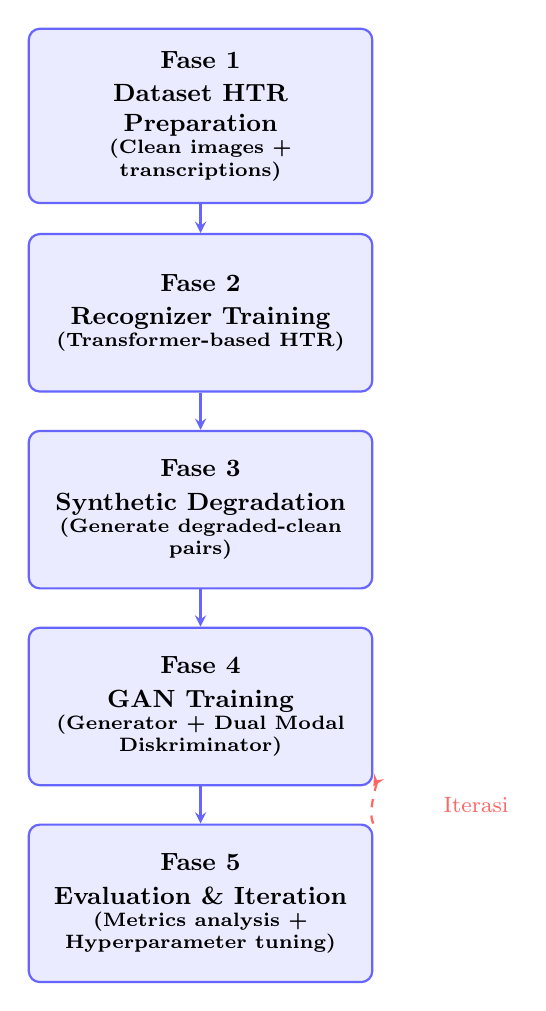
\begin{tikzpicture}[
    node distance=2cm,
    box/.style={
        rectangle,
        draw=blue!60,
        thick,
        minimum width=4.2cm,
        minimum height=2cm,
        text centered,
        font=\small\bfseries,
        fill=blue!8,
        rounded corners=4pt,
        inner sep=8pt
    },
    arrow/.style={
        ->,
        thick,
        >=stealth,
        color=blue!60
    }
]

% Phase 1
\node[box] (phase1) at (0,0) {
    \begin{minipage}{3.8cm}
    \centering
    \textbf{Fase 1}\\
    \vspace{0.1em}
    Dataset HTR Preparation\\
    \scriptsize{(Clean images + transcriptions)}
    \end{minipage}
};

% Phase 2
\node[box] (phase2) at (0,-2.5) {
    \begin{minipage}{3.8cm}
    \centering
    \textbf{Fase 2}\\
    \vspace{0.1em}
    Recognizer Training\\
    \scriptsize{(Transformer-based HTR)}
    \end{minipage}
};

% Phase 3
\node[box] (phase3) at (0,-5) {
    \begin{minipage}{3.8cm}
    \centering
    \textbf{Fase 3}\\
    \vspace{0.1em}
    Synthetic Degradation\\
    \scriptsize{(Generate degraded-clean pairs)}
    \end{minipage}
};

% Phase 4
\node[box] (phase4) at (0,-7.5) {
    \begin{minipage}{3.8cm}
    \centering
    \textbf{Fase 4}\\
    \vspace{0.1em}
    GAN Training\\
    \scriptsize{(Generator + Dual Modal Diskriminator)}
    \end{minipage}
};

% Phase 5
\node[box] (phase5) at (0,-10) {
    \begin{minipage}{3.8cm}
    \centering
    \textbf{Fase 5}\\
    \vspace{0.1em}
    Evaluation \& Iteration\\
    \scriptsize{(Metrics analysis + Hyperparameter tuning)}
    \end{minipage}
};

% Arrows
\draw[arrow] (phase1.south) -- (phase2.north);
\draw[arrow] (phase2.south) -- (phase3.north);
\draw[arrow] (phase3.south) -- (phase4.north);
\draw[arrow] (phase4.south) -- (phase5.north);

% Iteration arrow with label
\draw[arrow, dashed, thick, color=red!60, bend right=35]
    (phase5.north east) to[out=30, in=-30] (phase4.south east);
\node[font=\footnotesize, color=red!60] at (3.5,-8.75) {Iterasi};

\end{tikzpicture}
\caption{Pipeline pengembangan framework GAN-HTR dengan lima fase utama yang dilakukan secara sekuensial dengan iterasi pada fase 4 dan 5.}
\label{fig:development-pipeline}
\end{figure}

\subparagraph{Fase 1: Persiapan Dataset HTR}

Dataset bersih disiapkan untuk melatih model Recognizer dengan struktur:
\begin{itemize}[leftmargin=*, nosep]
\item \textbf{Input:} Gambar line text bersih (1024$\times$128 piksel, grayscale)
\item \textbf{Label:} Ground truth transcription dalam format UTF-8
\item \textbf{Format:} TFRecord untuk efisiensi loading
\item \textbf{Sumber:} Koleksi dokumen historis Arsip Nasional RI yang telah ditranskrip manual
\item \textbf{Preprocessing:} Normalisasi intensitas, padding, resizing
\end{itemize}

Lokasi dataset: \texttt{real\_data\_preparation/real\_data.tfrecord}

Charlist: \texttt{real\_data\_preparation/real\_data\_charlist.txt}

\subparagraph{Fase 2: Pelatihan dan Pembekuan Recognizer}

Model Recognizer dilatih menggunakan arsitektur Transformer-based HTR:

\textit{Arsitektur:}
\begin{itemize}[leftmargin=*, nosep]
\item Encoder: CNN untuk ekstraksi fitur visual (output: sequence of feature vectors)
\item Decoder: Transformer dengan multi-head attention untuk sequence-to-sequence mapping
\item Output: Probabilitas karakter per timestep, loss dihitung dengan CTC
\end{itemize}

\textit{Training Configuration:}
\begin{itemize}[leftmargin=*, nosep]
\item Optimizer: Adam dengan learning rate $1 \times 10^{-4}$
\item Batch size: 16
\item Epochs: Hingga konvergen (monitoring CER pada validation set)
\item Early stopping: Patience 10 epochs tanpa improvement pada validation CER
\end{itemize}

Setelah training, bobot model recognizer dibekukan (\textit{frozen}) untuk digunakan sebagai evaluator objektif selama training GAN. Filosofi ini memastikan bahwa CTC loss yang dihitung selama training GAN mencerminkan keterbacaan intrinsik gambar hasil restorasi, bukan pergeseran target karena recognizer yang juga sedang belajar.

Model terbaik tersimpan di: \texttt{models/best\_htr\_recognizer/best\_model.weights.h5}

\subparagraph{Fase 3: Synthetic Degradation Pipeline}

Karena keterbatasan ketersediaan data berpasangan (degraded-clean) untuk dokumen historis, dikembangkan pipeline degradasi sintetis yang realistis untuk menghasilkan training pairs dari dokumen bersih.

\textit{Jenis Degradasi yang Disimulasikan:}

\begin{table}[H]
\centering
\caption{Parameter degradasi sintetis}
\label{tab:synthetic-degradation}
\small
\begin{tabular}{|l|p{6cm}|p{4cm}|}
\hline
\textbf{Jenis} & \textbf{Metode Implementasi} & \textbf{Parameter} \\ \hline
Bleed through & Alpha blending dengan background noise texture & Alpha: 0.3-0.7 \\ \hline
Fading & Reduksi kontras dengan gamma correction & Gamma: 1.5-2.5 \\ \hline
Stains & Perlin noise overlay dengan color shift & Intensity: 0.2-0.5 \\ \hline
Blur & Gaussian blur dengan varying kernel & Sigma: 1.0-3.0 \\ \hline
Salt \& Pepper Noise & Random pixel corruption & Density: 0.01-0.05 \\ \hline
\end{tabular}
\end{table}

Pipeline degradasi diimplementasikan dalam Python dengan OpenCV dan diintegrasikan dalam data augmentation pipeline TensorFlow. Setiap gambar bersih diproses dengan kombinasi acak dari degradasi di atas dengan probabilitas tertentu untuk mensimulasikan variasi natural dokumen historis.

Output: Dataset triplet (degraded image, clean image, ground truth text) dalam format TFRecord.

Lokasi: \texttt{dual\_modal\_gan/data/dataset\_gan.tfrecord}

Dokumentasi lengkap proses: \texttt{DOKUMENTASI/LAPORAN\_PEMBUATAN\_DATASET\_SINTETIS\_BARU.md}

\subsubsection{Detail Implementasi Framework}
\label{subsubsec:detail-implementasi}

\paragraph{Lingkungan Eksperimen}
Seluruh proses eksperimen, mulai dari persiapan data, training model, hingga evaluasi, dijalankan pada lingkungan dengan spesifikasi sebagai berikut:

\textbf{Perangkat Keras:}
Komputasi utama dijalankan pada workstation yang dilengkapi dengan unit pemrosesan grafis (GPU) NVIDIA RTX A4000. Pemanfaatan GPU secara signifikan mempercepat proses training model deep learning yang intensif secara komputasi.

\textbf{Perangkat Lunak:}
\begin{itemize}
    \item \textbf{Sistem Operasi:} Linux
    \item \textbf{Bahasa Pemrograman:} Python 3.10
    \item \textbf{Manajemen Lingkungan:} Seluruh dependensi dan paket Python dikelola menggunakan Poetry untuk memastikan reproduktifitas lingkungan kerja
\end{itemize}

\textbf{Library Utama:}
\begin{itemize}
    \item \textbf{TensorFlow (v2.x):} Digunakan sebagai kerangka kerja utama untuk membangun, melatih, dan mengevaluasi seluruh model deep learning
    \item \textbf{NumPy:} Digunakan secara ekstensif untuk manipulasi data numerik dan array
    \item \textbf{OpenCV (cv2):} Digunakan untuk tugas-tugas pemrosesan gambar pada tahap persiapan data
    \item \textbf{Tqdm:} Digunakan untuk memberikan visualisasi progress bar yang informatif
\end{itemize}

\paragraph{Pipeline Persiapan Dataset}
Fondasi dari penelitian ini adalah dataset yang berkualitas tinggi dan dirancang secara spesifik. Mengingat kelangkaan dataset publik yang menyediakan pasangan gambar dokumen historis terdegradasi dan versi bersihnya beserta transkripsi akurat, pendekatan yang diambil adalah membangun dataset secara mandiri.

\textbf{Fase 1: Pembuatan Dataset Ground Truth untuk Recognizer (HTR)}
Tujuan dari fase ini adalah untuk membangun dataset dasar yang bersih dan terverifikasi untuk melatih model Recognizer (HTR). Proses pembuatannya melibatkan:

\begin{enumerate}
    \item \textbf{Segmentasi dan Anotasi Halaman:} Proses dimulai dari pindaian digital dokumen arsip utuh. Peneliti melakukan segmentasi dan anotasi pada setiap halaman untuk mengidentifikasi batas-batas setiap baris teks. Hasil adalah file Page-XML yang mendefinisikan koordinat geometris dan konten tekstual untuk setiap baris.

    \item \textbf{Ekstraksi Pasangan Data Mentah:} Berdasarkan informasi Page-XML, skrip otomatis mengekstrak setiap baris teks dengan cropping gambar baris individual dan mengambil transkripsi sebagai label.

    \item \textbf{Pembersihan dan Binarisasi Gambar:} Gambar baris teks diekstraksi dibersihkan menggunakan DE-GAN dalam mode inferensi untuk menciptakan ground truth visual yang seragam dan berstandar tinggi.

    \item \textbf{Verifikasi dan Kurasi Final:} Prosedur validasi memastikan setiap gambar bersih memiliki pasangan label yang tepat.

    \item \textbf{Pengemasan Data:} Dataset dikemas dalam format TFRecord untuk optimasi I/O selama training.
\end{enumerate}

\textbf{Fase 2: Pembuatan Dataset Triplet Sintetis untuk Training GAN}
Setelah model Recognizer dilatih dan dibekukan, fase kedua berfokus pada pembuatan dataset GAN dengan data triplet (gambar terdegradasi, gambar bersih, label teks).

Pipeline degradasi sintetis mensimulasikan berbagai jenis degradasi:
\begin{itemize}
    \item \textbf{Bleed Through:} Alpha blending dengan background noise texture (Alpha: 0.3-0.7)
    \item \textbf{Fading:} Reduksi kontras dengan gamma correction (Gamma: 1.5-2.5)
    \item \textbf{Stains:} Perlin noise overlay dengan color shift (Intensity: 0.2-0.5)
    \item \textbf{Blur:} Gaussian blur dengan varying kernel (Sigma: 1.0-3.0)
    \item \textbf{Salt \& Pepper Noise:} Random pixel corruption (Density: 0.01-0.05)
\end{itemize}

\paragraph{Konfigurasi Training dan Hyperparameter}
\textbf{Generator Training Configuration:}
\begin{itemize}
    \item Optimizer: Adam dengan learning rate $1 \times 10^{-4}$
    \item Batch size: 16 (adjustable berdasarkan GPU memory)
    \item Loss components: Adversarial loss (1.0), L1 reconstruction loss (100.0), CTC readability loss (1.0)
    \item Gradient clipping: clipnorm=1.0 untuk mencegah exploding gradients
\end{itemize}

\textbf{Diskriminator Training Configuration:}
\begin{itemize}
    \item Optimizer: Adam dengan learning rate $5 \times 10^{-4}$
    \item Loss: Binary cross-entropy dengan label smoothing
    \item Target accuracy: 60-80\% (Nash equilibrium zone)
\end{itemize}

\textbf{Stabilitas Training Strategies:}
\begin{itemize}
    \item \textbf{Pure FP32 Precision:} Menghindari numerical instability dari FP16 mixed precision
    \item \textbf{Gradient Clipping:} Mencegah exploding gradients dengan clipnorm=1.0
    \item \textbf{Learning Rate Scheduling:} Reduksi learning rate ketika validation loss plateau
    \item \textbf{Early Stopping:} Patience 10 epochs tanpa improvement pada validation CER
\end{itemize}

\paragraph{Sistem Evaluasi Komprehensif}
\textbf{Metrik Visual:}
\begin{itemize}
    \item \textbf{PSNR (Peak Signal-to-Noise Ratio):} Mengukur kesamaan piksel dengan ground truth. Target: $>$ 35 dB
    \item \textbf{SSIM (Structural Similarity Index):} Mengukur kesamaan struktural. Target: $>$ 0.95
\end{itemize}

\textbf{Metrik Tekstual:}
\begin{itemize}
    \item \textbf{CER (Character Error Rate):} Rasio karakter yang salah dikenali. Target: Penurunan minimal 30\% vs baseline
    \item \textbf{WER (Word Error Rate):} Rasio kata yang salah dikenali. Target: Penurunan signifikan vs baseline
\end{itemize}

\textbf{Combined Score untuk Balanced Objective:}
\begin{equation}
\text{Combined Score} = \alpha \cdot \text{PSNR}_{norm} + \beta \cdot \text{SSIM} + \gamma \cdot (1 - \text{CER})
\end{equation}
dengan $\alpha = 0.3$, $\beta = 0.3$, $\gamma = 0.4$ untuk menyeimbangkan antara kualitas visual dan keterbacaan teks.

\subparagraph{Fase 4: Implementasi dan Training GAN}

Framework GAN dengan komponen utama:

\textit{1. Generator (U-Net Architecture)}

Arsitektur encoder-decoder dengan skip connections untuk preservasi detail spasial:

\begin{itemize}[leftmargin=*, nosep]
\item \textbf{Encoder:} 5 blok downsampling (Conv2D + LeakyReLU + BatchNorm)
\begin{itemize}[nosep]
\item Input: 1024$\times$128$\times$1
\item Features: 64 $\rightarrow$ 128 $\rightarrow$ 256 $\rightarrow$ 512 $\rightarrow$ 512
\item Downsampling: Stride 2 pada Conv2D
\end{itemize}

\item \textbf{Bottleneck:} Dense feature representation (32$\times$4$\times$512)

\item \textbf{Decoder:} 5 blok upsampling (Conv2DTranspose + ReLU + BatchNorm)
\begin{itemize}[nosep]
\item Features: 512 $\rightarrow$ 512 $\rightarrow$ 256 $\rightarrow$ 128 $\rightarrow$ 64
\item Upsampling: Stride 2 pada Conv2DTranspose
\item Skip connections: Concatenation dari encoder features
\end{itemize}

\item \textbf{Output Layer:} Conv2D (1$\times$1 kernel) dengan Tanh activation
\begin{itemize}[nosep]
\item Output: 1024$\times$128$\times$1 (restored image)
\end{itemize}
\end{itemize}

Justifikasi U-Net: Skip connections memungkinkan gradient flow langsung dari decoder ke encoder, mencegah vanishing gradient problem dan mempertahankan detail fine-grained seperti stroke karakter yang krusial untuk keterbacaan HTR.

\textit{2. Dual Modal Diskriminator}

Inovasi utama penelitian ini adalah diskriminator dengan dua cabang evaluasi:

\textit{Visual Branch (CNN):}
\begin{itemize}[leftmargin=*, nosep]
\item Input: Concatenation (degraded image, restored/real image)
\item Architecture: 5 Conv2D layers dengan stride 2 (downsampling)
\item Features: 64 $\rightarrow$ 128 $\rightarrow$ 256 $\rightarrow$ 512 $\rightarrow$ 1024
\item Output: Visual feature vector (flattened dari final conv layer)
\end{itemize}

\textit{Text Branch (LSTM):}
\begin{itemize}[leftmargin=*, nosep]
\item Input: HTR features dari frozen recognizer (sequence of feature vectors)
\item Architecture: Bidirectional LSTM dengan 256 units
\item Purpose: Mengevaluasi koherensi sekuensial teks yang terbaca dari gambar
\item Output: Text feature vector (final LSTM hidden state)
\end{itemize}

\textit{Fusion Layer:}
\begin{itemize}[leftmargin=*, nosep]
\item Concatenation visual features dan text features
\item Dense layers: 512 $\rightarrow$ 256 $\rightarrow$ 1
\item Final activation: Sigmoid (real/fake probability)
\end{itemize}

Justifikasi Dual Modal: Dengan mengevaluasi gambar dari dua perspektif (visual realism dan text coherence), diskriminator memberikan sinyal yang lebih kaya kepada generator, mendorong output yang tidak hanya terlihat realistis tetapi juga mudah dibaca oleh HTR.

\begin{figure}[H]
\centering
% TODO: Insert diagram dual modal diskriminator detail
% File: images/dual_modal_detail.png
\fbox{\parbox{0.9\textwidth}{\centering
\textbf{[PLACEHOLDER GAMBAR III.3]}\\[0.5em]
Detail Arsitektur Dual Modal Diskriminator:\\[0.3em]
Input: Degraded Image + Restored/Real Image\\[-0.1em]
        $\downarrow$                    $\downarrow$\\[-0.1em]
[Visual Branch - CNN]     [Frozen Recognizer]\\[-0.1em]
Conv2D layers (5)         Extract HTR features\\[-0.1em]
64-128-256-512-1024       Feature sequence\\[-0.1em]
        $\downarrow$                    $\downarrow$\\[-0.1em]
Flatten: 1024-dim         [Text Branch - LSTM]\\[-0.1em]
                          BiLSTM 256 units\\[-0.1em]
        $\downarrow$                    $\downarrow$\\[-0.1em]
   Visual Features        Text Features\\[-0.1em]
        $\downarrow$                    $\downarrow$\\[-0.1em]
           [Concatenation]\\[-0.1em]
                  $\downarrow$\\[-0.1em]
           Dense 512 $\rightarrow$ 256\\[-0.1em]
                  $\downarrow$\\[-0.1em]
           Output: Real/Fake (0-1)\\[0.3em]
\textit{Innovation: Joint visual-textual evaluation}
}}
\caption{Detail arsitektur Dual Modal Diskriminator menunjukkan aliran data melalui dua cabang paralel dan fusion layer untuk keputusan akhir.}
\label{fig:dual-modal-detail}
\end{figure}

\textit{3. Multi-Component Loss Function}

Generator dilatih dengan tiga komponen loss:

\textbf{(a) Adversarial Loss:}
\begin{equation}
\mathcal{L}_{adv} = - \mathbb{E}_{x \sim p_{data}(x)}[\log D(x, G(x))]
\end{equation}

Mendorong generator menghasilkan gambar yang dapat menipu diskriminator (dinilai sebagai ``real''). Menggunakan Binary Cross Entropy dengan label smoothing (real label: 0.9, fake label: 0.1) untuk stabilitas training.

\textbf{(b) L1 Reconstruction Loss:}
\begin{equation}
\mathcal{L}_{L1} = \mathbb{E}_{x, y \sim p_{data}(x,y)}[\|y - G(x)\|_1]
\end{equation}

Memastikan gambar hasil restorasi $G(x)$ mendekati ground truth clean image $y$ secara pixel wise. L1 loss dipilih dibanding L2 (MSE) karena lebih robust terhadap outlier dan menghasilkan gambar yang lebih tajam.

\textbf{(c) CTC Loss (HTR-Oriented):}
\begin{equation}
\mathcal{L}_{CTC} = - \log P(l | R(G(x)))
\end{equation}

di mana $R$ adalah frozen recognizer, $G(x)$ adalah restored image, dan $l$ adalah ground truth transcription. CTC loss mengukur seberapa mudah recognizer dapat membaca teks dari gambar hasil restorasi. Komponen loss ini adalah inovasi kunci yang membedakan penelitian ini dari metode sebelumnya.

\textbf{Total Generator Loss:}
\begin{equation}
\mathcal{L}_G = \lambda_{adv} \mathcal{L}_{adv} + \lambda_{L1} \mathcal{L}_{L1} + \lambda_{CTC} \mathcal{L}_{CTC}
\end{equation}

dengan weight balancing:
\begin{itemize}[leftmargin=*, nosep]
\item $\lambda_{adv} = 1.0$ (realisme visual)
\item $\lambda_{L1} = 100.0$ (content preservation, bobot tinggi karena skala loss kecil)
\item $\lambda_{CTC} = 1.0$ (text readability)
\end{itemize}

Weight ini dipilih berdasarkan eksperimen awal dan disesuaikan jika diperlukan berdasarkan analisis training dynamics.

\textbf{Diskriminator Loss:}

Standar binary cross entropy untuk real/fake classification:
\begin{equation}
\mathcal{L}_D = - \mathbb{E}_{x,y}[\log D(x,y)] - \mathbb{E}_{x}[\log(1 - D(x, G(x)))]
\end{equation}

\textit{4. Training Configuration}

\begin{table}[H]
\centering
\caption{Konfigurasi training GAN}
\label{tab:training-config}
\small
\begin{tabular}{|l|l|}
\hline
\textbf{Parameter} & \textbf{Nilai} \\ \hline
Optimizer & Adam ($\beta_1=0.5$, $\beta_2=0.999$) \\ \hline
Learning Rate (Generator) & $2 \times 10^{-4}$ \\ \hline
Learning Rate (Diskriminator) & $2 \times 10^{-4}$ \\ \hline
Batch Size & 8 (constraint GPU memory) \\ \hline
Epochs & 100 (dengan early stopping) \\ \hline
Precision & FP32 (Pure Float32 untuk stabilitas) \\ \hline
GPU & 1x NVIDIA RTX A4000 (16 GB) \\ \hline
Training Strategy & Alternating (1 D step, 1 G step) \\ \hline
Gradient Clipping & Norm = 1.0 (prevent exploding gradient) \\ \hline
\end{tabular}
\end{table}

Justifikasi FP32: Setelah eksperimen dengan Mixed Precision (FP16), ditemukan bahwa training lebih stabil dengan Pure FP32 meskipun lebih lambat. Gradient pada CTC loss cenderung memiliki skala yang sangat kecil dan rentan terhadap underflow pada FP16.

\textit{5. Monitoring dan Logging}

Setiap eksperimen dilacak menggunakan MLflow dengan metadata:
\begin{itemize}[leftmargin=*, nosep]
\item Hyperparameters: Loss weights, learning rates, batch size
\item Metrics: G loss, D loss, D accuracy, PSNR, SSIM, CER, WER (per epoch)
\item Artifacts: Model checkpoints, sample restored images, training curves
\item Git commit: Untuk reproduktifitas kode
\end{itemize}

Dokumentasi integrasi MLflow: \texttt{logbook/MLFLOW\_INTEGRATION.md}

\subparagraph{Fase 5: Eksperimen dan Iterasi Berbasis Bukti}

Pengembangan framework dilakukan melalui siklus iteratif dengan eksperimen terkontrol:

\textit{Eksperimen 1: Diskriminator Mode Comparison}

\textbf{Pertanyaan:} Apakah text branch sebaiknya menggunakan predicted transcription dari recognizer atau ground truth transcription?

\textbf{Metode:} Ultra-fast comparison dengan training singkat (5 epochs) pada kedua mode.

\textbf{Hasil:} Mode \texttt{ground\_truth} menunjukkan konvergensi lebih stabil dan PSNR lebih tinggi. Mode \texttt{predicted} menyebabkan instabilitas karena recognizer errors propagate ke diskriminator signal.

\textbf{Keputusan:} Adopsi mode \texttt{ground\_truth} untuk training final.

Dokumentasi: \texttt{logbook/ANALYSIS\_ultrafast\_comparison\_results.md}

\textit{Eksperimen 2: Loss Weight Tuning}

\textbf{Pertanyaan:} Bagaimana weight $\lambda_{L1}$ dan $\lambda_{CTC}$ mempengaruhi trade-off antara visual quality dan text readability?

\textbf{Metode:} Grid search pada nilai $\lambda_{L1} \in \{50, 100, 150\}$ dan $\lambda_{CTC} \in \{0.5, 1.0, 2.0\}$.

\textbf{Hasil:} $\lambda_{L1}=100$ dan $\lambda_{CTC}=1.0$ memberikan keseimbangan optimal dengan PSNR $>$ 35 dB dan CER reduction $>$ 30\%.

Dokumentasi: \texttt{logbook/FIX\_training\_configuration\_20251005.md}

\textit{Eksperimen 3: Training Anomaly Analysis}

\textbf{Masalah:} Loss generator stagnan pada epoch tertentu, diskriminator accuracy terlalu tinggi ($>$ 95\%).

\textbf{Analisis:} Diskriminator terlalu kuat, generator tidak mendapat sinyal gradient yang cukup informatif.

\textbf{Solusi:} (1) Label smoothing pada diskriminator, (2) Penurunan learning rate diskriminator menjadi $1 \times 10^{-4}$, (3) Gradient clipping pada diskriminator.

Dokumentasi: \texttt{logbook/ANALYSIS\_training\_anomalies\_20251005.md}

\subsubsection{Tahap 4: Demonstrasi}
\label{subsubsec:demonstrasi}

Artefak yang telah dikembangkan didemonstrasikan untuk menunjukkan kemampuannya dalam menyelesaikan masalah restorasi dokumen terdegradasi dan meningkatkan keterbacaan HTR.

\textbf{Studi Kasus:}

Penerapan model final pada sampel data uji yang representatif:

\begin{table}[H]
\centering
\caption{Rencana demonstrasi framework}
\label{tab:demo-plan}
\small
\begin{tabular}{|l|p{5cm}|p{5cm}|}
\hline
\textbf{Dataset} & \textbf{Karakteristik} & \textbf{Tujuan} \\ \hline
Synthetic Test Set & Degradasi terkontrol dengan ground truth & Evaluasi kuantitatif objektif \\ \hline
DIBCO Benchmark & Dataset publik untuk binarization & Komparasi dengan metode lain \\ \hline
Real ANRI Documents & Dokumen historis asli dari Arsip Nasional & Validasi pada degradasi nyata \\ \hline
\end{tabular}
\end{table}

\textbf{Visualisasi Hasil:}

Untuk setiap sampel, dihasilkan visualisasi perbandingan:
\begin{itemize}[leftmargin=*, nosep]
\item Input: Degraded image
\item Output: Restored image (hasil dari Generator)
\item Reference: Clean ground truth (jika tersedia)
\item Overlay: Difference heatmap untuk menunjukkan area yang direstorasi
\end{itemize}

Visualisasi disimpan sebagai artifact di MLflow dengan metadata (PSNR, SSIM, predicted text, ground truth text, CER).

\textbf{Demonstration Metrics:}

Selain metrik kuantitatif, dilakukan evaluasi kualitatif:
\begin{itemize}[leftmargin=*, nosep]
\item Preservasi struktur karakter (tidak ada distorsi yang merusak keterbacaan)
\item Konsistensi restorasi (tidak ada artefak checkerboard atau blotching)
\item Generalisasi (performa pada jenis degradasi yang tidak terlihat saat training)
\end{itemize}

\subsubsection{Tahap 5: Evaluasi}
\label{subsubsec:evaluasi}

Tahap ini mengukur performa artefak secara objektif terhadap tujuan yang telah didefinisikan dan memvalidasi hipotesis penelitian.

\textbf{Evaluasi Kuantitatif:}

\textit{1. Metrik Visual Quality}

Menghitung PSNR dan SSIM pada validation set:

\textbf{PSNR (Peak Signal to Noise Ratio):}
\begin{equation}
PSNR = 10 \log_{10} \left( \frac{MAX_I^2}{MSE} \right)
\end{equation}

di mana $MAX_I$ adalah nilai maksimum pixel (255 untuk 8-bit image) dan $MSE$ adalah Mean Squared Error antara ground truth dan restored image.

\textbf{SSIM (Structural Similarity Index):}
\begin{equation}
SSIM(x, y) = \frac{(2\mu_x\mu_y + C_1)(2\sigma_{xy} + C_2)}{(\mu_x^2 + \mu_y^2 + C_1)(\sigma_x^2 + \sigma_y^2 + C_2)}
\end{equation}

di mana $\mu$ adalah mean, $\sigma$ adalah standard deviation, $\sigma_{xy}$ adalah covariance, dan $C_1, C_2$ adalah konstanta stabilitas.

\textit{2. Metrik Text Readability}

Menghitung CER dan WER menggunakan frozen recognizer:

\textbf{CER (Character Error Rate):}
\begin{equation}
CER = \frac{S + D + I}{N} \times 100\%
\end{equation}

di mana $S$ adalah substitutions, $D$ adalah deletions, $I$ adalah insertions, dan $N$ adalah jumlah karakter ground truth.

\textbf{WER (Word Error Rate):}
\begin{equation}
WER = \frac{S_w + D_w + I_w}{N_w} \times 100\%
\end{equation}

dengan definisi analog pada level kata.

\textit{3. Combined Score}

Untuk memberikan evaluasi holistik, dikembangkan combined score:
\begin{equation}
Score = 0.3 \times PSNR_{norm} + 0.3 \times SSIM + 0.4 \times (1 - CER)
\end{equation}

di mana $PSNR_{norm}$ adalah PSNR dinormalisasi ke range [0, 1] dengan threshold 50 dB sebagai nilai maksimum. Bobot 0.4 pada komponen CER mencerminkan prioritas pada keterbacaan teks.

\textbf{Perbandingan dengan Baseline:}

\begin{table}[H]
\centering
\caption{Target perbandingan evaluasi kuantitatif}
\label{tab:eval-target}
\small
\begin{tabular}{|l|c|c|c|}
\hline
\textbf{Metode} & \textbf{PSNR (dB)} & \textbf{SSIM} & \textbf{CER (\%)} \\ \hline
No Restoration (Baseline) & N/A & N/A & High \\ \hline
DE-GAN & $\sim$38 & $>$0.90 & Not reported \\ \hline
U-Net (L1 only) & $\sim$32 & $\sim$0.89 & Medium \\ \hline
\textbf{Ours (Proposed)} & \textbf{$>$35} & \textbf{$>$0.95} & \textbf{Significantly reduced} \\ \hline
\end{tabular}
\end{table}

\textbf{Analisis Statistik:}

Untuk memvalidasi signifikansi improvement:
\begin{itemize}[leftmargin=*, nosep]
\item Paired t-test untuk membandingkan metrik (PSNR, SSIM, CER) antara metode proposed dan baseline
\item Effect size (Cohen's d) untuk mengukur magnitude of improvement
\item Confidence interval 95\% untuk setiap metrik
\end{itemize}

\textbf{Validasi Hipotesis:}

Mengevaluasi hipotesis penelitian yang diajukan di Bab I:

\textbf{H$_0$} (Null Hypothesis): Tidak ada perbedaan signifikan antara metode proposed dan baseline dalam hal keterbacaan teks (CER).

\textbf{H$_1$} (Alternative Hypothesis): Metode proposed menghasilkan CER yang signifikan lebih rendah dibandingkan baseline dengan confidence level 95\%.

Kriteria penolakan H$_0$: p-value $<$ 0.05 dari paired t-test.

\textbf{Validasi Integritas Data:}

Dilakukan asesmen untuk memastikan tidak ada data leakage:
\begin{itemize}[leftmargin=*, nosep]
\item Verifikasi bahwa training set dan validation set tidak overlap
\item Verifikasi bahwa synthetic degradation tidak menggunakan pattern yang terlalu sederhana (risiko overfitting)
\item Cross-validation dengan k-fold (k=5) untuk mengukur variance performa
\end{itemize}

Dokumentasi: \texttt{logbook/DATA\_LEAKAGE\_ASSESSMENT.md}

\textbf{Analisis Failure Cases:}

Identifikasi dan analisis sampel di mana model gagal (CER tinggi atau PSNR rendah):
\begin{itemize}[leftmargin=*, nosep]
\item Karakteristik visual yang menyebabkan kegagalan (degradasi ekstrem, font unik, etc.)
\item Pattern errors dari recognizer (character confusions)
\item Usulan improvement untuk iterasi berikutnya
\end{itemize}

\subsubsection{Tahap 6: Komunikasi}
\label{subsubsec:komunikasi}

Hasil penelitian dan artefak yang dihasilkan dikomunikasikan kepada komunitas ilmiah dan praktisi untuk diseminasi pengetahuan dan mendorong reproduktifitas.

\textbf{Penulisan Tesis:}

Mendokumentasikan seluruh proses penelitian dalam format tesis yang terstruktur:
\begin{itemize}[leftmargin=*, nosep]
\item \textbf{Bab I (Pendahuluan):} Konteks, motivasi, rumusan masalah, tujuan, hipotesis, kontribusi
\item \textbf{Bab II (Tinjauan Pustaka):} State of the art, gap analysis, theoretical foundation
\item \textbf{Bab III (Metodologi):} DSRM framework, tahapan penelitian, tools dan environment
\item \textbf{Bab IV (Analisis dan Desain):} Spesifikasi teknis arsitektur, implementasi detail
\item \textbf{Bab V (Hasil dan Pembahasan):} Eksperimen, evaluasi kuantitatif, analisis hasil
\item \textbf{Bab VI (Kesimpulan dan Saran):} Ringkasan temuan, jawaban RQ, future work
\end{itemize}

\textbf{Publikasi Ilmiah:}

Menyiapkan manuscript untuk publikasi di venue ilmiah:

\textit{Target Journal:} IEEE Transactions on Pattern Analysis and Machine Intelligence (TPAMI) atau International Journal on Document Analysis and Recognition (IJDAR) (Q1 journal).

\textit{Struktur Paper:}
\begin{itemize}[leftmargin=*, nosep]
\item Abstract: Ringkasan problem, novelty, hasil
\item Introduction: Motivation dan contribution
\item Related Work: Brief literature review dengan focus pada gap
\item Methodology: Dual Modal Diskriminator dan HTR-oriented loss
\item Experiments: Dataset, metrics, comparison dengan state of the art
\item Results: Quantitative dan qualitative analysis
\item Conclusion: Summary dan future directions
\end{itemize}

\textit{Novelty yang Ditekankan:}
\begin{itemize}[leftmargin=*, nosep]
\item Dual Modal Diskriminator architecture (first to jointly evaluate visual and text features)
\item HTR-oriented loss integration (explicit CTC loss dalam training GAN)
\item Frozen recognizer philosophy (objective evaluation of text readability)
\item Superior performance pada dokumen dengan degradasi kompleks
\end{itemize}

\textbf{Open Source dan Reproduktifitas:}

Membagikan artefak penelitian untuk transparansi dan kemajuan sains:

\textit{GitHub Repository:}
\begin{itemize}[leftmargin=*, nosep]
\item Source code: \texttt{train32.py}, \texttt{models/}, \texttt{dual\_modal\_gan/}
\item Documentation: README lengkap, installation guide, usage examples
\item Pretrained models: Best checkpoint untuk reproduksi hasil
\item Dataset: Synthetic degradation scripts (bukan raw data karena copyright ANRI)
\item License: Apache 2.0 atau MIT untuk encourage adoption
\end{itemize}

\textit{MLflow Artifacts:}
\begin{itemize}[leftmargin=*, nosep]
\item Tracking server public (jika memungkinkan) untuk transparency
\item Export eksperimen logs dalam format yang portable (CSV, JSON)
\end{itemize}

\textit{Logbook Publication:}

Semua hasil analisis training dan eksperimen di folder \texttt{logbook/} disusun sebagai supplementary materials yang dapat diakses untuk peer review dan validasi.

\textbf{Presentasi dan Disseminasi:}

\begin{itemize}[leftmargin=*, nosep]
\item Presentasi hasil pada seminar internal ITB
\item Presentasi pada konferensi internasional (ICDAR, DAS, atau CVPR workshop)
\item Kolaborasi dengan Arsip Nasional RI untuk implementasi praktis
\item Workshop atau tutorial untuk komunitas digital humanities dan archival science
\end{itemize}

\subsection{Alat dan Lingkungan Eksperimen}
\label{subsec:tools-environment}

Bagian ini merinci spesifikasi teknis dari lingkungan yang digunakan untuk penelitian, memastikan transparansi dan reproduktifitas.

\subsubsection{Perangkat Keras}
\label{subsubsec:hardware}

\begin{table}[H]
\centering
\caption{Spesifikasi perangkat keras}
\label{tab:hardware-spec}
\small
\begin{tabular}{|l|l|}
\hline
\textbf{Komponen} & \textbf{Spesifikasi} \\ \hline
GPU & NVIDIA RTX A4000 (16 GB GDDR6) \\ \hline
CPU & Intel Xeon atau AMD Ryzen (multi-core) \\ \hline
RAM & 32 GB DDR4 \\ \hline
Storage & 1 TB NVMe SSD (untuk dataset dan checkpoints) \\ \hline
\end{tabular}
\end{table}

Justifikasi: GPU dengan 16 GB memory diperlukan untuk batch size 8 pada resolusi 1024$\times$128 dengan model yang complex (Generator + Diskriminator + Recognizer features). Training dengan 1 GPU (ALLOW\_GPU=1) untuk stabilitas dan menghindari NaN issues.

\subsubsection{Perangkat Lunak}
\label{subsubsec:software}

\begin{table}[H]
\centering
\caption{Framework deep learning dan library utama}
\label{tab:software-framework}
\small
\begin{tabular}{|l|l|l|}
\hline
\textbf{Kategori} & \textbf{Tool/Library} & \textbf{Versi} \\ \hline
Language & Python & 3.10 \\ \hline
Deep Learning Framework & TensorFlow/Keras & 2.x \\ \hline
Dependency Management & Poetry & Latest \\ \hline
Numerical Computing & NumPy & Latest \\ \hline
Image Processing & OpenCV & 4.x \\ \hline
Experiment Tracking & MLflow & 2.x \\ \hline
Visualization & Matplotlib, Seaborn & Latest \\ \hline
\end{tabular}
\end{table}

\begin{table}[H]
\centering
\caption{Manajemen data dan augmentasi}
\label{tab:data-management}
\small
\begin{tabular}{|l|l|}
\hline
\textbf{Aspek} & \textbf{Tool/Method} \\ \hline
Dataset Format & TFRecord (untuk efisiensi loading) \\ \hline
Data Pipeline & \texttt{tf.data.Dataset} dengan prefetch dan cache \\ \hline
Augmentation & Custom degradation pipeline dengan OpenCV \\ \hline
Versioning & Git untuk code, MLflow untuk data artifacts \\ \hline
\end{tabular}
\end{table}

\subsubsection{Infrastruktur dan Kolaborasi}
\label{subsubsec:infrastructure}

\begin{table}[H]
\centering
\caption{Infrastruktur pengembangan}
\label{tab:infrastructure}
\small
\begin{tabular}{|l|l|}
\hline
\textbf{Komponen} & \textbf{Detail} \\ \hline
Version Control & Git (GitHub repository: GAN-HTR-ORI) \\ \hline
Experiment Tracking & MLflow dengan local tracking server \\ \hline
Documentation & Markdown files dalam \texttt{logbook/} folder \\ \hline
Code Editor & VS Code dengan Python extensions \\ \hline
Containerization & Docker (untuk deployment dan reproducibility) \\ \hline
\end{tabular}
\end{table}

\subsubsection{Testing dan Evaluasi}
\label{subsubsec:testing}

\begin{table}[H]
\centering
\caption{Tools untuk testing dan evaluasi}
\label{tab:testing-tools}
\small
\begin{tabular}{|l|l|}
\hline
\textbf{Aspek} & \textbf{Method/Tool} \\ \hline
Unit Testing & pytest untuk testing individual components \\ \hline
Smoke Testing & Eksperimen cepat (5 epochs) sebelum full training \\ \hline
Metric Calculation & Custom scripts untuk PSNR, SSIM, CER, WER \\ \hline
Statistical Analysis & SciPy untuk t-test dan confidence intervals \\ \hline
Visualization & Custom plotting scripts dengan Matplotlib \\ \hline
\end{tabular}
\end{table}

\subsection{Manajemen Penelitian}
\label{subsec:research-management}

\subsubsection{Prinsip Penelitian}
\label{subsubsec:research-principles}

Penelitian ini mengikuti prinsip-prinsip berikut untuk memastikan kualitas dan integritas:

\textbf{1. Don't Repeat Yourself (DRY):} Kode yang reusable dan modular untuk menghindari duplikasi dan mempermudah maintenance.

\textbf{2. Smoke Test First:} Sebelum training skala penuh, selalu lakukan smoke test dengan dataset kecil atau epochs sedikit untuk validasi pipeline dan deteksi bugs early.

\textbf{3. Documentation Driven:} Setiap temuan, eksperimen, atau bug fix didokumentasikan dalam \texttt{logbook/} dengan timestamp untuk tracking progress dan learning.

\textbf{4. Clean Slate Training:} Sebelum training, hapus checkpoint yang bermasalah untuk menghindari carry-over errors.

\textbf{5. Deep Inspection Before Action:} Sebelum membuat perubahan signifikan, lakukan inspeksi mendalam kode dan data untuk memahami root cause masalah.

\subsubsection{Dokumentasi Logbook}
\label{subsubsec:logbook-documentation}

Semua hasil training, analisis, dan decision making tercatat dalam folder \texttt{logbook/} dengan struktur:

\begin{center}
\ttfamily
logbook/\\\relax
|-- ANALYSIS\_ultrafast\_comparison\_results.md\\\relax
|-- ANALYSIS\_training\_anomalies\_20251005.md\\\relax
|-- FIX\_training\_configuration\_20251005.md\\\relax
|-- DATA\_LEAKAGE\_ASSESSMENT.md\\\relax
|-- MLFLOW\_INTEGRATION.md\\\relax
`-- [timestamp]\_[topic].md
\end{center}

Setiap file mengikuti template:
\begin{itemize}[leftmargin=*, nosep]
\item \textbf{Date:} Timestamp
\item \textbf{Objective:} Tujuan analisis atau eksperimen
\item \textbf{Method:} Cara yang digunakan
\item \textbf{Results:} Temuan utama dengan metrics dan visualizations
\item \textbf{Conclusions:} Interpretasi dan decision
\item \textbf{Next Actions:} Follow-up yang diperlukan
\end{itemize}

\subsection{Timeline dan Milestones}
\label{subsec:timeline}

\begin{table}[H]
\centering
\caption{Timeline penelitian dengan milestones}
\label{tab:timeline}
\small
\begin{tabular}{|l|l|p{6cm}|}
\hline
\textbf{Fase} & \textbf{Durasi} & \textbf{Deliverables} \\ \hline
Fase 1: Preparation & 2 bulan & Dataset HTR, Recognizer trained \\ \hline
Fase 2: Development & 3 bulan & GAN framework implemented dan tested \\ \hline
Fase 3: Experimentation & 2 bulan & Iterasi eksperimen, hyperparameter tuning \\ \hline
Fase 4: Evaluation & 1 bulan & Comprehensive evaluation, statistical analysis \\ \hline
Fase 5: Writing & 2 bulan & Thesis draft dan paper manuscript \\ \hline
\textbf{Total} & \textbf{10 bulan} & \textbf{Complete thesis dan publication ready paper} \\ \hline
\end{tabular}
\end{table}

\subsection{Kesimpulan Bab}
\label{subsec:kesimpulan-bab}

Bab ini telah menguraikan metodologi penelitian yang komprehensif berdasarkan Design Science Research Methodology (DSRM) dengan enam tahapan yang saling terkait: identifikasi masalah, definisi tujuan, desain dan pengembangan, demonstrasi, evaluasi, dan komunikasi. Setiap tahapan dijelaskan secara detail dengan metode, tools, dan dokumentasi yang digunakan.

Pendekatan iteratif berbasis bukti memastikan bahwa setiap keputusan desain dan hyperparameter didukung oleh eksperimen terkontrol dan analisis data. Framework GAN dengan Dual Modal Diskriminator dan HTR-oriented loss function dikembangkan melalui siklus penyempurnaan berkelanjutan dengan monitoring ketat menggunakan MLflow dan dokumentasi sistematis dalam logbook.

Metodologi ini dirancang untuk memastikan:
\begin{enumerate}[leftmargin=*, nosep]
\item \textbf{Reproduktifitas:} Semua eksperimen terlacak dengan MLflow, kode tersimpan di Git dengan commit hash
\item \textbf{Transparansi:} Setiap decision didokumentasikan dengan justifikasi berbasis data
\item \textbf{Rigor:} Evaluasi menggunakan metrik standar dan statistical significance testing
\item \textbf{Impact:} Hasil dikomunikasikan melalui publikasi ilmiah dan open source untuk benefit komunitas
\end{enumerate}

Bab berikutnya (Bab IV) akan menguraikan analisis dan desain teknis framework secara mendetail, termasuk spesifikasi arsitektur, algoritma training, dan implementasi pipeline data.

\end{document}
